\documentclass{article}
\usepackage[utf8]{inputenc}
\usepackage{blindtext}
\usepackage{graphicx}
\usepackage{listings}
\usepackage{subfig}
\title{\Huge{BBC Micro:bit pedometer task}}
\author{William Smith}
\begin{document}
\maketitle{}
\section{Introduction - \textit{"Hello World"}}
In this task you'll be using the official JavaScript block editor to turn the BBC Micro:bit into a pedometer; a pedometer is a step counter. Below is an example of what the website looks like and it can be found by entering \textbf{"https://makecode.microbit.org/"} into your Internet browser.
\begin{center}
	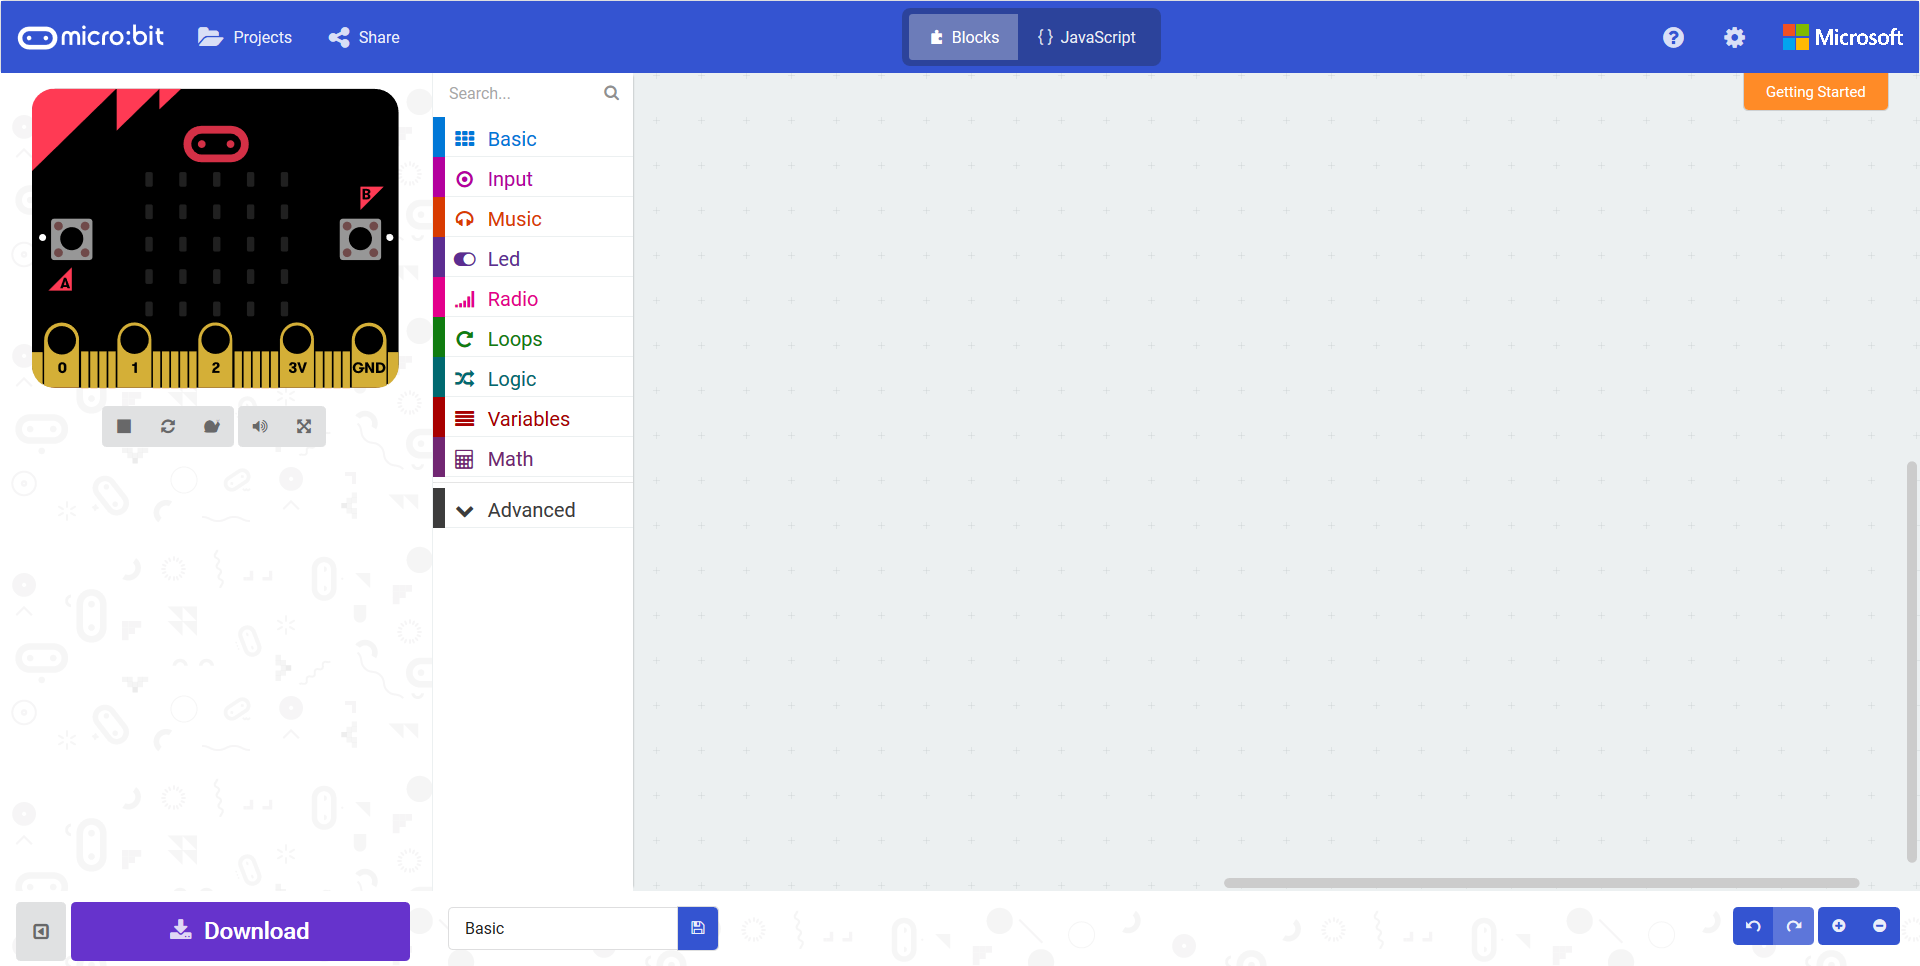
\includegraphics[scale=0.15]{blockedit}
\end{center}
The block editor allows you to easily drag and drop commands to develop simple (and some more complex) programs without dealing with annoying errors. If you have ever used the program scratch the block editor is very similar; Scratch's logo can be found in Figure \ref{fig:scratch}.
\begin{figure}
  \centering
    
\includegraphics[scale=0.3]{scratch}
  \caption{The logo for Scratch}
  \label{fig:scratch}
\end{figure}
\newpage
\section{The Main Part}
The main part of the task is the counting of steps taken. This will be done using the input block for run on shake (as shown in the image below)
\begin{center}
	
\includegraphics[scale=1]{Onshake}
\end{center}
You'll also need a variable (let's say its called steps) to store the number of steps. The valuable should be increased by 1 when the device is shook.
\begin{center}
	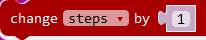
\includegraphics[scale=1]{Steps}
\end{center}
You should also have some way of seeing if the code is actually working; To do this you can have an image flash on the screen when a step is taken. You will need to use the show icon, pause and clear commands for this (the clear is so that you can obviously see when a step is taken).
\begin{figure}[!hp]
  \centering
  \subfloat[Pause Command]{
\includegraphics[width=0.4\textwidth]{pause}\label{fig:f1}}
  \hfill
  \subfloat[Clear Command]{
\includegraphics[width=0.4\textwidth]{clearscreen}\label{fig:f2}}
  \hfill
  \subfloat[Show Icon Command]{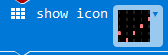
\includegraphics[width=0.4\textwidth]{showicon}\label{fig:f3}}
  \caption{The three commands}
\end{figure}
\newpage
You can now download the code and upload it to the Micro:bit. To do this you must first download it using the button in the bottom left-hand corner (as shown below).
\begin{figure}[!hp]
  \centering
    
\includegraphics[scale=0.5]{download}
  \label{fig:download}
\end{figure}

Once you have downloaded your .hex file navigate to the folder that it is in. Then, connect your Micro:bit to the computer using the cable. Right-click on the .hex file and select send to and then Micro:bit. The file should copy across and start running.
\begin{center}
	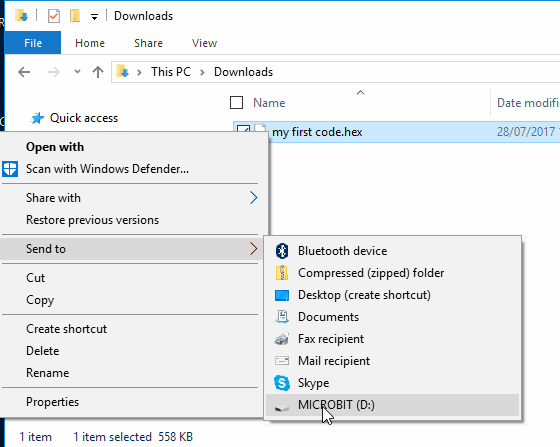
\includegraphics[scale=0.7]{sendto}
\end{center}
\newpage
\section{Show steps and reset}
\subsection{Showing Steps Taken}
It's important for the user to actually be able to see how many steps they have taken. For this you can use the "run on" command once again, however, this time it will run when the A button is pressed. You also need to use the "show number" command (make sure the number isn't a random one; you can find the steps variable by itself to do this).
\begin{figure}[!hp]
  \centering
  \subfloat["Show Number"]{
\includegraphics[width=0.4\textwidth]{shownum}\label{fig:shownum}}
  \hfill
  \subfloat["Set variable to"]{
\includegraphics[width=0.4\textwidth]{stepsolo}\label{fig:solo}}
  \caption{The two commands}
\end{figure}
\subsection{Resetting the Step Counter}
To reset the step counter you'll be using the "run on" and the "set variable to" command (Examples of these are shown in Figure 4); You may also want to show the user that the steps have been reset by using the "show number command is Figure 3)
\begin{figure}[!hp]
  \centering
  \subfloat["Run on B"]{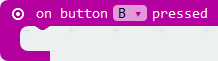
\includegraphics[width=0.4\textwidth]{onb}\label{fig:onb}}
  \hfill
  \subfloat["Set variable to"]{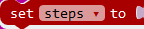
\includegraphics[width=0.4\textwidth]{set0}\label{fig:set0}}
  \caption{The two commands}
\end{figure}


Once you have added both these steps you can do the same procedure you did last time to install them on the Micro:bit and test to see if they work.
\end{document}